%% LaTeX-Beamer template for KIT design
%% by Erik Burger, Christian Hammer
%% title picture by Klaus Krogmann
%%
%% version 2.1
%%
%% mostly compatible to KIT corporate design v2.0
%% http://intranet.kit.edu/gestaltungsrichtlinien.php
%%
%% Problems, bugs and comments to
%% burger@kit.edu

\documentclass[18pt]{beamer}
\usepackage[utf8x]{inputenc}
\usepackage{units}
\usepackage{booktabs}

%% CUSTOM
\usepackage{amsmath}
\usepackage{algpseudocode}

%% Definitions
\DeclareMathOperator{\div2}{div}
\renewcommand{\algorithmicrequire}{\textbf{Input:}}
\renewcommand{\algorithmicensure}{\textbf{Output:}}
\algnewcommand\algorithmicto{\textbf{to}}
\algrenewtext{For}[3]{\algorithmicfor\ $#1 \gets #2$ \algorithmicto\ $#3$ \algorithmicdo}
\algnewcommand\algorithmicod{\textbf{od}}
\algrenewtext{EndWhile}{\algorithmicod}
\algrenewtext{EndFor}{\algorithmicod}
%\AtBeginSection[]{%
%\begin{frame}<beamer> % do nothing in handouts
%    \frametitle{Überblick}
%    \tableofcontents[sectionstyle=show/shaded,
%    subsectionstyle=show/show/hide]
%\end{frame}
%}
%\AtBeginSubsection[]{%
%\begin{frame}<beamer> % do nothing in handouts
%    \frametitle{Überblick}
%    \tableofcontents[sectionstyle=show/shaded,
%    subsectionstyle=show/shaded/hide]
%\end{frame}
%}

%% SLIDE FORMAT

% use 'beamerthemekit' for standard 4:3 ratio
% for widescreen slides (16:9), use 'beamerthemekitwide'

\usepackage{templates/beamerthemekit}
%\usepackage{templates/beamerthemekitwide}

 %% TITLE PICTURE

 % if a custom picture is to be used on the title page, copy it into the 'logos'
 % directory, in the line below, replace 'mypicture' with the 
 % filename (without extension) and uncomment the following line
 % (picture proportions: 63 : 20 for standard, 169 : 40 for wide
 % *.eps format if you use latex+dvips+ps2pdf, 
 % *.jpg/*.png/*.pdf if you use pdflatex)


 \titleimage{banner}
 
 
%% Define some colors:
\definecolor{darkblue}{rgb}{0,0,.5}
\definecolor{darkgreen}{rgb}{0,.5,0}

 %% TITLE LOGO

 % for a custom logo on the front page, copy your file into the 'logos'
 % directory, insert the filename in the line below and uncomment it

\titlelogo{logo_150x150}
 
 % (*.eps format if you use latex+dvips+ps2pdf,
 % *.jpg/*.png/*.pdf if you use pdflatex)
 
 %% TikZ INTEGRATION
 
 % use these packages for PCM symbols and UML classes
 % \usepackage{templates/tikzkit}
 % \usepackage{templates/tikzuml}
 
 % the presentation starts here
 
\author{Dominik Muth - dominik.muth@student.kit.edu}
\institute{Institut f\"ur Informatik}

\subtitle{Foliensatz 10}
\date{10. Januar 2013}

\begin{document}

\begin{frame}
    \titlepage
\end{frame}

\begin{frame}{Outline/Gliederung}
    \tableofcontents
\end{frame}

\section{Wiederholung}
\begin{frame} {Wiederholung - Quiz}
    \begin{itemize}
        \item Aus $f\in \Omega(g) \land f \in \Theta(g) \Rightarrow f \in \mathcal{O}(g)$
        \only<2-> {\color{darkgreen}$\surd$}\\
        \color{black}
                
        \item $n^5 \in \mathcal{O}(2^n)$
        \only<3-> {\color{darkgreen}$\surd$}\\
        \color{black}

        \item $\frac{n^3+2n}{2n+1} \in \mathcal{O}(n)$
        \only<4-> {\color{red}$X$}\\
        \color{black}
        
        \item Alle Algorithmen liegen in $\Omega(1)$
        \only<5-> {\color{darkgreen}$\surd$}\\
        \color{black}
    \end{itemize}
\end{frame}
\section{Master-Theorem}
\begin{frame}{Master-Theorem}
    \begin{block}{Definition}
        Für einen \emph{rekursiven} Algorithmus der Form
        \begin{align*}
            T\left( n \right) = aT\left( \frac{n}{b} \right) + f\left( n \right)
        \end{align*}
        kann die Laufzeit für drei Fälle abgeschätzt werden:
        \pause
        \begin{enumerate}
            \item Wenn $f\left( n \right)\in \mathcal{O}\left( n^{\log_b a-\varepsilon} \right)$ für ein $\varepsilon > 0$, 
                dann ist $T\left( n \right) \in \Theta\left( n^{\log_b a} \right)$
                \pause
            \item Wenn $f\left( n \right)\in \Theta\left( n^{\log_b a} \right)$, 
                dann ist $T\left( n \right) \in \Theta\left( n^{\log_b a} \log n\right)$
                \pause
            \item Wenn $f\left( n \right)\in \Omega\left( n^{\log_b a+\varepsilon} \right)$ für ein $\varepsilon > 0$, \\ 
                und wenn es eine Konstante $d$ gibt mit $0<d<1$,\\ 
                sodass für alle hinreichend großen $n$ gilt $af\left( \nicefrac{n}{b} \right) \leq df\left( n \right)$,\\ 
                dann ist $T\left( n \right) \in \Theta\left( f\left( n \right) \right)$
        \end{enumerate}
    \end{block}
    \begin{itemize}
        \item Fall 2 wird etwa bei Quicksort benötigt
        \item Fall 3 ist eher die Ausnahme
    \end{itemize}
\end{frame}
\begin{frame}{Master Theorem}
    \begin{exampleblock}{Beispiele}
        \[49 \cdot T( \frac{n}{7} ) + 3n + 5\]\\
        \[49 \cdot T( \frac{n}{7} ) + 3n^3 + 5\]\\
    \end{exampleblock}
\end{frame}

\section{Mealy-Automat}
\begin{frame}{Mealy-Automat}
    \begin{block}{Definition: Mealy-Automat}
        Der Mealy-Automat $A = \left( Z, z_0, X, f, Y, g \right)$ besteht aus
        \begin{enumerate}
            \item der endlichen Zustandsmenge $\mathbf{Z}$,
            \item dem Startzustand $\mathbf{z_0}$,
            \item dem Eingabealphabet $\mathbf{X}$,
            \item der Zustandsübergangsfunktion $\mathbf{f: Z\times X \rightarrow Z}$,
            \item einem Ausgabealphabet $\mathbf{Y}$ und
            \item der Ausgabefunktion $\mathbf{g: Z\times X \rightarrow Y^*}$.
        \end{enumerate}
    \end{block}
\end{frame}
\begin{frame}{Getränkeautomat}
    \begin{figure}[htbp]
        \centering
        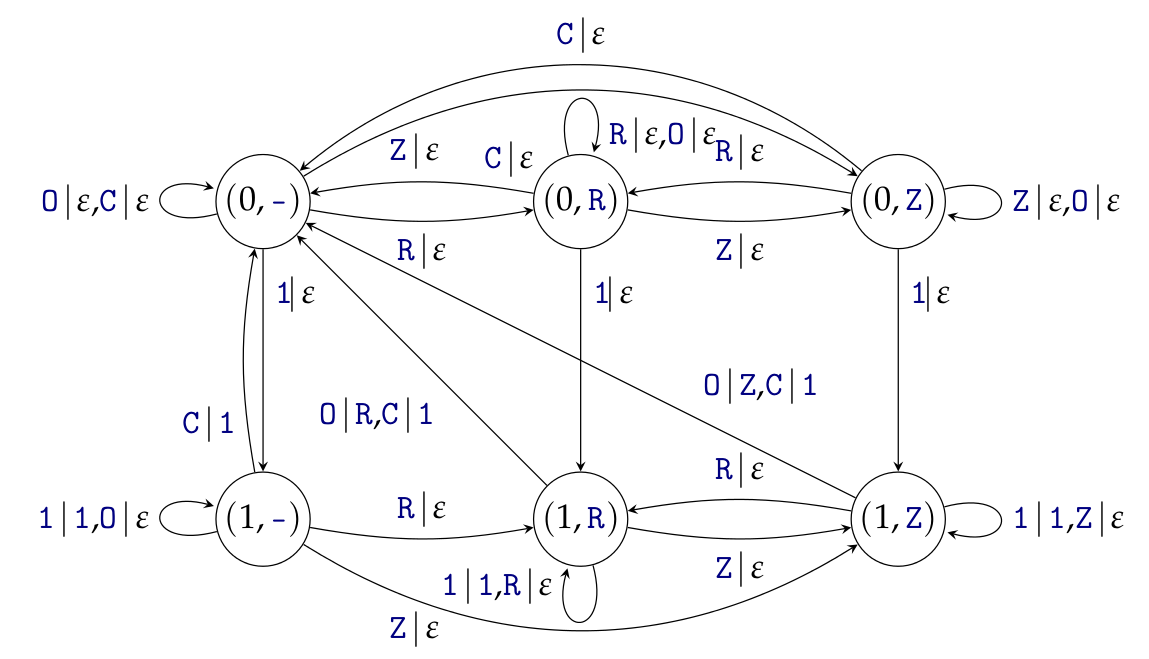
\includegraphics[width=\textwidth,height=\textheight,keepaspectratio]{graphics/10/getraenke2.png}
    \end{figure}
\end{frame}
\begin{frame}{Getränkeautomat}
    Was ist was?
    \begin{itemize}
        \item Zustandsmenge $Z$: \visible<2->{$\left\{ \left( 0,- \right), \left( 0,R \right), \left( 0,Z \right), \left( 1,- \right), \left( 1,R \right), \left( 1,Z \right) \right\}$}
            \pause
        \item Eingabealphabet $X$: \visible<3->{$\left\{ 1, R, Z, C, 0 \right\}$}
            \pause
        \item Zustandsübergangsfunktion $f$: \visible<4->{die Pfeile}
            \pause
        \item Ausgabealphabet $Y$: \visible<5->{$\left\{ 1, R, Z \right\}$}
            \pause
        \item Ausgabefunktion $g$: bisher noch nicht eingezeichnet, siehe nächste Folie
            \pause
    \end{itemize}
\end{frame}
\begin{frame}{Getränkeautomat (mit Ausgabe)}
    \begin{figure}[htbp]
        \centering
        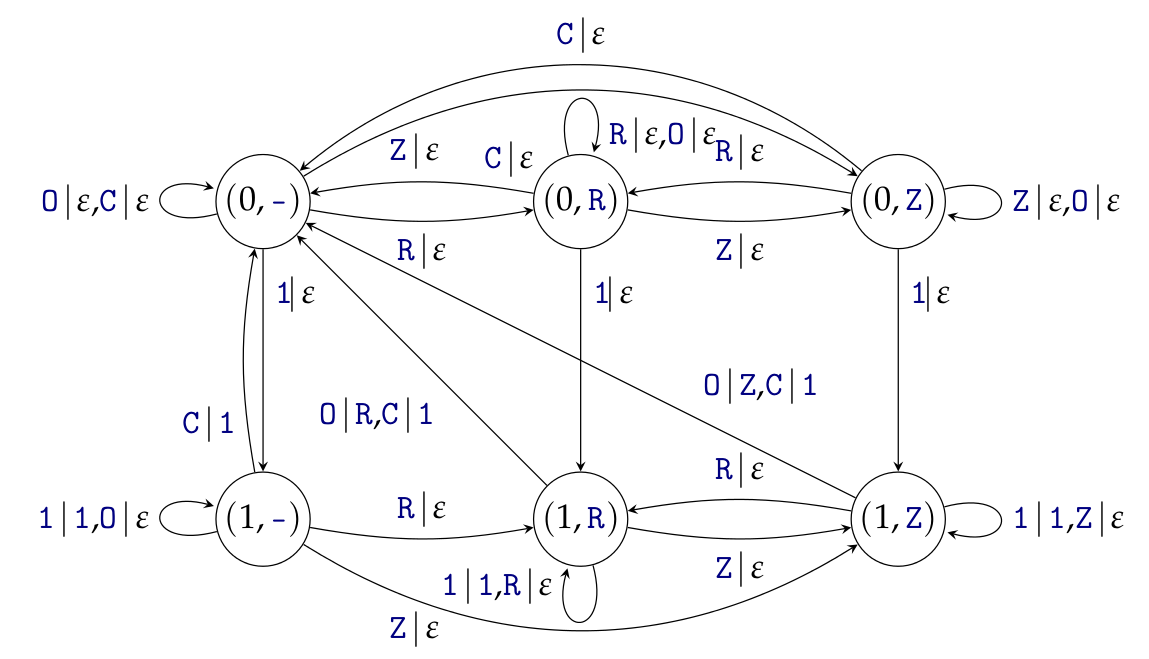
\includegraphics[width=\textwidth,height=\textheight,keepaspectratio]{graphics/10/getraenke2.png}
    \end{figure}
\end{frame}
\begin{frame}{Getränkeautomat}
    Was ist was?
    \begin{itemize}
        \item Zustandsmenge $Z$: $\left\{ \left( 0,- \right), \left( 0,R \right), \left( 0,Z \right), \left( 1,- \right), \left( 1,R \right), \left( 1,Z \right) \right\}$
        \item Eingabealphabet $X$: $\left\{ 1, R, Z, C, 0 \right\}$
        \item Zustandsübergangsfunktion $f$: die Pfeile, was vor einem senkrechten Strich $|$ steht
        \item Ausgabealphabet $Y$: $\left\{ 1, R, Z \right\}$
        \item Ausgabefunktion $g$: die Pfeile, was hinter einem senkrechten Strich $|$ steht
    \end{itemize}
\end{frame}
\begin{frame}{$f*$ und $f**$}
    \begin{block}{Definition: $f*$ und $f**$}
        $f^* = f^*\left( z,w \right)$ kann im Gegensatz zu $f$ ein ganzes Wort $w$ als zweites Funktionsargument nehmen: 
        \begin{align*}
            f^*: Z\times X^* &\rightarrow Z\\
            f^*\left( z, \varepsilon \right) &= z\\
            f^*\left( z, wx \right) &= f\left( f^*\left( z,w \right) ,x \right)
        \end{align*}
        \pause
        $f^{**}$ kann im Gegensatz zu $f^*$ ganze Wörter anstatt einem Symbol ausgeben:
        \begin{align*}
            f^{*}: Z\times X^* &\rightarrow Z^*\\
            f^{**}\left( z,\varepsilon \right) &= z\\
            \visible<2->{f^{**}\left( z, wx \right) &= f^{**}\left( z,w \right)\cdot f\left( f^*\left( z,w \right) ,x \right)}
        \end{align*}
    \end{block}
\end{frame}
\begin{frame}{Getränkeautomat (ohne Ausgabe)}
    \begin{figure}[htbp]
        \centering
        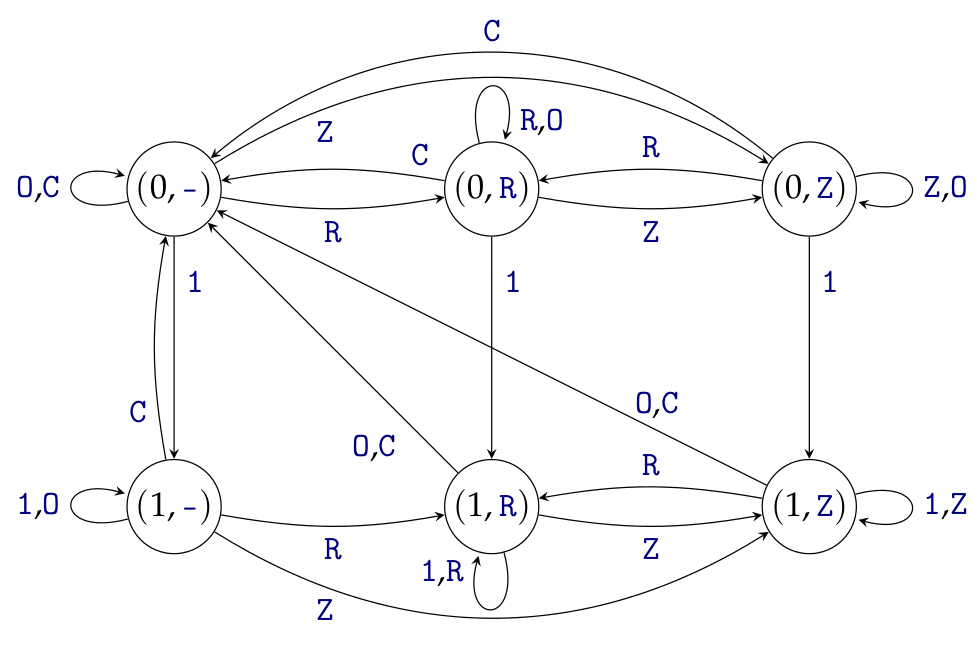
\includegraphics[width=.80\textwidth,height=.8\textheight,keepaspectratio]{graphics/10/getraenke.png}
    \end{figure}
    Was macht $f^*\left( \left( 0,- \right), R10 \right)$? \pause\visible<2->{Berechnet $f^*\left( \left( 0, - \right), R10 \right)$.} \pause \visible<3->{Was käme bei $f^{**}\left( \left( 0,- \right), R10 \right)$ raus?}
\end{frame}
\begin{frame}{Getränkeautomat (mit Ausgabe)}
    \begin{figure}[htbp]
        \centering
        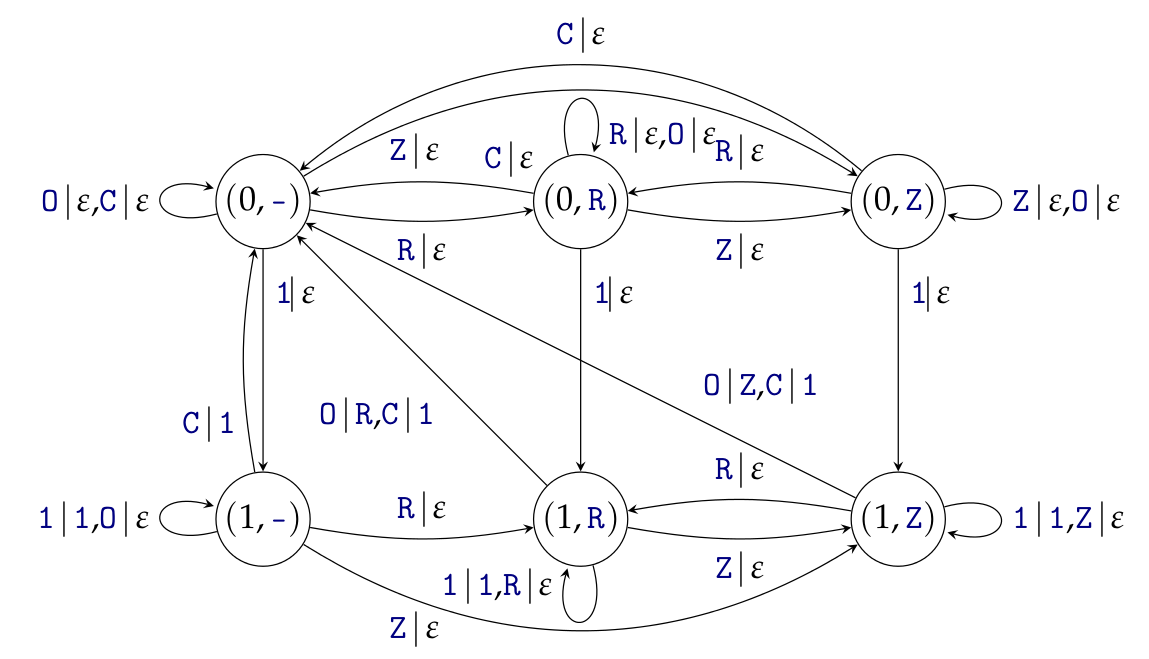
\includegraphics[width=.80\textwidth,height=.8\textheight,keepaspectratio]{graphics/10/getraenke2.png}
    \end{figure}
    Was macht $g^*\left( \left( 0,- \right), R10 \right)$? \pause\visible<2->{Berechnet $g^*\left( \left( 0, - \right), R10 \right)$.} \pause \visible<3->{Was käme bei $g^{**}\left( \left( 0,- \right), R10 \right)$ raus?} \pause \visible<4->{Was passiert bei $g^{**}\left( \left( 0, - \right), R110 \right) = 1R$}
\end{frame}
\begin{frame}{Alternativer Automat}
    Gegeben sei der Automat mit
    \begin{itemize}
        \item $Z = \left\{ z \right\}$,
        \item $X = Y = \left\{ a, b \right\}$,
        \item $g\left( z, a \right) = b$,
        \item $g\left( z, b \right) = ba$.
     \end{itemize}
     \begin{enumerate}
         \item Zeichnet den Automaten,
         \item gebt $w_1 = g^{**}\left( z, a \right)$ an und
         \item gebt $w_2 = g^{**}\left( z, w_1 \right)$ an.
     \end{enumerate}
     Wie sieht $w_3$ vermutlich aus? Allgemein, wie sieht $w_i$ aus?
\end{frame}
\begin{frame}{Alternativer Automat}
    \begin{figure}
    \centering
    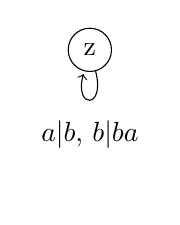
\begin{tikzpicture}
      \tikzstyle{every node}=[draw,shape=circle];
        \path[fill] (0,0)  node[circle] (0) {z};

        \path[->,draw] (0) edge [loop below] node[draw=none,below=-10pt]{ $a|b$, $b|ba$ } ();
    \end{tikzpicture}
    \end{figure}
    \begin{itemize}
        \item $w_1 = g^{**}\left( z, a \right) = g^{**}\left( z, \varepsilon \right)\cdot g^*\left( z, wx \right) = g\left( f^*\left( z, \varepsilon \right), a \right) = g\left( z, a \right) = b$
        \item $w_2 = \dots = ba$
    \end{itemize}
\end{frame}

\section{Moore-Automat}
\begin{frame}{Moore-Automaten}
    \begin{block}{Definition: Mealy-Automat}
        Der Mealy-Automat $A = \left( Z, z_0, X, f, Y, h \right)$ besteht aus
        \pause
        \visible<2->{\begin{enumerate}
            \item der endlichen Zustandsmenge $\mathbf{Z}$,
            \item dem Startzustand $\mathbf{z_0}$,
            \item dem Eingabealphabet $\mathbf{X}$,
            \item der Zustandsübergangsfunktion $\mathbf{f: Z\times X \rightarrow Z}$,
            \item einem Ausgabealphabet $\mathbf{Y}$ und
            \item \color{red}{der Ausgabefunktion $\mathbf{h: Z \rightarrow Y^*}$.}
        \end{enumerate}}
    \end{block}
    Bis auf die Asgabefunktion sind Mealy- und Moore-Automat identisch. Der Moore-Automat hat seine Ausgabe in einem Zustand.
\end{frame}

\section{Endliche Akzeptoren}
\begin{frame}{Endlicher Akzeptor}
    \begin{block}{Definition: Endlicher Akzeptor}
        Ein endlicher Akzepter ist ein spezieller Moore-Automat, der 
        \begin{itemize}
            \item $1$ ausgibt, wenn ein Wort einer Wortbildungsregel (Syntax) entspricht und
            \item $0$ ansonsten ausgibt.
        \end{itemize}
        \pause
        Im Gegensatz zum gewöhnlichen Moore Automat besitzt er
        \begin{itemize}
            \item \emph{keine Ausgabefunktion $h$}, 
            \item dafür eine \emph{eine Menge $F \subseteq Z$ akzeptierender Zustände}.
        \end{itemize}
        \begin{align*}
            A = \left( Z, z_0, X, f, F \right)
        \end{align*}
    \end{block}
    Die akzeptierenden Zustände werden doppelt umrahmt.
\end{frame}
\begin{frame}{Endlicher Akzeptor: Beispiel}
    \begin{figure}[htbp]
        \centering
        \includegraphics[width=.80\textwidth,height=.8\textheight,keepaspectratio]{graphics/10/akzeptor.png}
    \end{figure}
    Nennt Wörter und sagt, ob diese akzeptiert werden oder nicht.
\end{frame}
\begin{frame}{Endlicher Akzeptor: Aufgabe}
    \begin{itemize}
        \item Gesucht ist ein kleiner endlicher Akzeptor, der alle Wörter akzeptiert, bei denen die Anzahl der $a$ durch $5$ teilbar ist.\\
            Gegeben: $X = \left\{ a,b \right\}$.
        \item Gesucht ist ein endlicher Akzeptor, in dem nirgends hintereinander zwei $b$ vorkommen.
    \end{itemize}
\end{frame}
\begin{frame}{Lösung 1}
    \begin{figure}
    \centering
    \begin{tikzpicture}
      \tikzstyle{every node}=[/tikz/initial text=];
        \path[fill] (0,0)  node[initial,state,accepting] (0) {0};
        \path[fill] (2,0)  node[state] (1) {1};
        \path[fill] (4,0)  node[state] (2) {2};
        \path[fill] (6,0)  node[state] (3) {3};
        \path[fill] (8,0)  node[state] (4) {4};

        \path[->] 
        (0) edge node[above] {a} (1)
        (1) edge node[above] {a} (2)
        (2) edge node[above] {a} (3)
        (3) edge node[above] {a} (4)
        (4) edge[bend right] node[above] {a} (0)

        (0) edge [loop below] node[below]{ b } ()
        (1) edge [loop below] node[below]{ b } ()
        (2) edge [loop below] node[below]{ b } ()
        (3) edge [loop below] node[below]{ b } ()
        (4) edge [loop below] node[below]{ b } ();
    \end{tikzpicture}
    \end{figure}
\end{frame}
\begin{frame}{Lösung 2}
    \begin{figure}
    \centering
    \begin{tikzpicture}
      \tikzstyle{every node}=[/tikz/initial text=];
        \path[fill] (0,0)  node[initial,state,accepting] (0) {0};
        \path[fill] (2,0)  node[state, accepting] (1) {1};
        \path[fill] (4,0)  node[state] (2) {2};

        \path[->] 
        (0) edge[bend right] node[below] {b} (1)
        (1) edge[bend right] node[above] {a} (0)
        (1) edge node[above] {b} (2)

        (0) edge [loop below] node[below]{ a } ()
        (2) edge [loop below] node[below]{ a,b } ();
    \end{tikzpicture}
    \end{figure}
\end{frame}
\end{document}
